\documentclass[12pt]{AlgebraQual}
\usepackage{preamble}

\name{Kayla Orlinsky}
\course{Algebra Exam}
\term{Spring 2018}
\hwnum{Spring 2018}

\begin{document}

\begin{problem} $\,$
Prove that a group of order $72$ cannot be simple.
\end{problem}


\begin{solution}$\,$
Let $G$ be a group of order $72$. Note that $72=9\cdot8=3^2\cdot 2^3$. Now, by the Sylow Theorems, $n_3\equiv 1\mod 3$ and $n_3|8$, so $n_3=1,4$.

Assume $G$ is simple. By the Sylow Theorems, Sylow $3$-subgroups are conjugates and $G$ can act on $\syl_3(G)$ the set of Sylow $3$ subgroups by conjugation. Note that since $n_3\not=1$, $n_3=4$ and so $|\syl_3(G)|=4$.

This induces a homomorphism $\varphi:G\to S_4$ where $\varphi(g)=\sigma_g$ which is the conjugation map \begin{align*}
    \sigma_g:\syl_3(G)&\to\syl_3(G)\\
    P_3&\mapsto gP_3g^{-1}
\end{align*}

Since $G$ is simple, $\ker\varphi$ must be trivial, since kernels are normal subgroups.

However, then $S_4$ has an isomorphic copy of $G$ inside it, which is not possible since $|S_4|=4!=24<|G|=72$.

This is a contradiction and so $G$ cannot be simple.

***Note that $n_3=4$ could still be possible, however, in this case, the kernel of the homomorphism induced by the conjuation action cannot be trivial.
\end{solution}
\newpage


\begin{problem} $\,$
Say that a group $G$ is uniquely $p$-divisible if the $p$-th power map sending $x\in G$ to $x^p$ is bijective. Show that if $G$ is a finitely generated uniquely $p$-divisible \textit{abelian} group, then $G$ is finite and has order coprime to $p.$
\end{problem}


\begin{solution}$\,$
Assume $G$ is abelian and finitely generated. Then by the fundamental theorem of finitely generated abelian groups, $$G\cong\mathbb{Z}^n\oplus(\mathbb{Z}_{p_1^{\alpha_1}})^{n_1}\oplus\cdots\oplus(\mathbb{Z}_{p_k^{\alpha_k}})^{n_k}$$ where $p_i$ are primes, and the $\alpha_i$ are distinct.

Now, $G$ is uniquely $p$ divisible, and so if $\varphi_p$ is the $p\thh$ power map, then $\varphi_p$ is bijective. However, this is only possible if $\varphi_p$ is bijective in each coordinate.

Let $\pi_l$ be the projection homorphism to the $l\thh$ coordinate.

However, then we can restrict $\varphi_p$ to the $l\thh$ coordinate to get that $\pi_l\circ\varphi_p|_{l\thh\text{ coordinate}}$ is also bijective for all $l$.

Since $\varphi_p$ is certainly not a surjective map restricted to $\mathbb{Z}$, $n=0$. Namely, $|G|<\infty.$

Furthermore, restricting to an automorphism of $\mathbb{Z}_{p_i^{\alpha_i}}$, we immediately get that $p\not=p_i$. Else, there would exist an element $x$ of order $p$ in $\mathbb{Z}_{p_i^{\alpha_i}}$ and so $\varphi_p(x)=x^p=e$. making $\varphi_p$ not injective on that coordinate.

Thus, $p\not=p_i$ for all $i$, and so $G$ must have order coprime to $p$.
\end{solution}
\newpage



\begin{problem} $\,$
Let $\mathbb{Q}$ be the field of rational numbers and consider $f(x)=x^8+x^4+1\in\mathbb{Q}[x].$ Write $E$ for a splitting field for $f(x)$ over $\mathbb{Q}$ and set $G=\gal(E/\mathbb{Q}).$ Find $|E:\mathbb{Q}|$ and determine the Galois group $G$ up to isomorphism. If $\Omega\subset E$ is the set of roots of $f(x)$, find the number of orbits for the action of $G$ on $\Omega$.
\end{problem}


\begin{solution}$\,$
Let $u=x^4$. Then $f(u)=u^2+u+1$, so \begin{align*}
    u^2+u+1&=0\\
    \implies u&=\frac{-1\pm\sqrt{1-4}}{2}\\
    &=\frac{-1\pm\sqrt{3}i}{2}\\
    &=e^{i2\pi/3},e^{i4\pi/3}
\end{align*}

Now, if $u$ is a root of $u^2+u+1$, then $x$ is a $4\thh$ root of $u$. At this point, we can note that the roots are all distinct and so $E$ is the splitting field of a separable polynomial so it is a Galois extension of $\mathbb{Q}$ and so $G=\gal(E/\mathbb{Q})$ exists.

Now, $\xi=e^{i\pi/6}$ is a primitive root of $e^{i2\pi/3}$ since the four roots are $$\xi=e^{i\pi/6},\xi^4=e^{i2\pi/3},\xi^7=e^{i7\pi/6},\xi^{10}=e^{5i\pi/3}$$ and since $(e^{2i\pi/3})^2=e^{i4\pi/3}$, we have that $\xi$ actually generates all the roots of $f(x)$. Now, we note two things, first, if $z$ is a root of $f(x)$ then $-z$ is also a root. Furthermore, if $z$ is a root, then $\overline{z}$ is also a root. Thus, starting with $u$ and $\overline{u}$, we can get that the roots are
\begin{center}
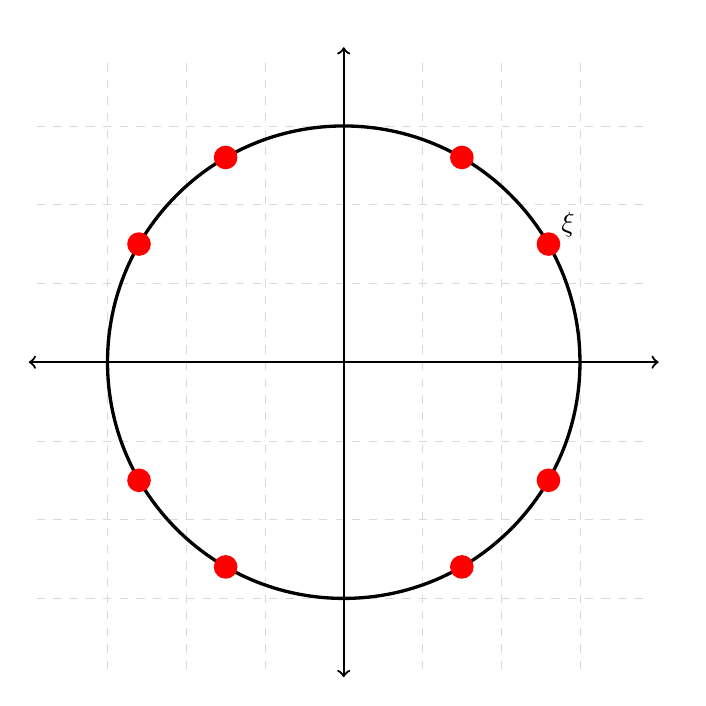
\begin{tikzpicture}
\draw[help lines, color=gray!30, dashed] (-3.9,-3.9) grid (3.9,3.9);
\draw[->,very thick] (0,0) circle (3cm);
\fill[very thick,red] (-2.6,-1.5) circle (0.15cm);
\fill[very thick,red] (2.6,-1.5) circle (0.15cm);
\fill[very thick,red] (-2.6,1.5) circle (0.15cm);
\draw (2.6,1.5) -- (2.6,1.5)  node[xshift=0.25cm,yshift=0.25cm]{$\xi$};
\fill[very thick,red] (2.6,1.5) circle (0.15cm);
\fill[very thick,red] (-1.5,-2.6) circle (0.15cm);
\fill[very thick,red] (-1.5,2.6) circle (0.15cm);
\fill[very thick,red] (1.5,-2.6) circle (0.15cm);
\fill[very thick,red] (1.5,2.6) circle (0.15cm);
\draw[<->, thick] (-4,0)--(4,0) node[right]{$\re$};
\draw[<->, thick] (0,-4)--(0,4) node[above]{$\im$};
\end{tikzpicture}
\end{center}

Namely, the roots are $$\xi,\xi^2,\xi^4,\xi^5,\xi^7,\xi^8,\xi^{10},\xi^{11}.$$

Therefore, $E=\mathbb{Q}(\xi)$. Now, $\xi^6=-1$ and so $\xi$ satisfies $g(x)=x^6+1$ \begin{align*}
    x^6+1&=(x^2)^3+1\\
    &=(x^2+1)(x^4-x^2+1)
\end{align*} since $\xi$ does not satisfy $x^2+1$, it must satisfy $x^4-x^2+1$, which is irreducible over $\mathbb{Q}$ by the quadratic formula.
Therefore, $$[E:\mathbb{Q}]=4.$$

Thus, by the Fundamenal Theorem of Galois theory, $|G|=4$. Since there are only two groups of order $4$ up to isomorphism, $G$ is abelian and it is either isomorphic to $\mathbb{Z}_2\times\mathbb{Z}_2$ or $\mathbb{Z}_4$.

Finally, we check whether $G$ has any elements of order $4$.

Let $\sigma,\tau\in G$ be defined by $\sigma(\xi)=\overline{\xi}$ and $\tau(\xi)=-\xi$. Both of these are clearly well defined by the computation for the roots of $f$ and both maps have order $2$, so if they are not equal, then $G$ must be $\mathbb{Z}_2\times\mathbb{Z_2}$ since $\mathbb{Z}_4$ has only one element of order $4.$ However, $$\overline{\xi}=e^{-i\pi/6}=e^{11i\pi/6}\qquad -\xi=e^{i(\pi/6+\pi)}=e^{i7\pi/6}$$ and these are clearly not equal, so $$G=\{\id,\sigma,\tau,\sigma\tau\}\cong\mathbb{Z}_2\times\mathbb{Z}_2.$$

Finally, using the image or via direct calculation, we see that the orbits are exactly $\{\xi^i,\sigma\cdot\xi^i,\tau\cdot\xi^i,\sigma\tau\cdot\xi^i\}$ where the action is defined by $g\cdot \xi^i=g(\xi^i)$ for $g\in G$.

Now, since $\tau$ fixes

has $2$ orbits, namely $$\{\xi,\xi^5,\xi^7,\xi^{11}\}\qquad \{\xi^2,\xi^4,\xi^8,\xi^{10}\}.$$
\end{solution}
\newpage




\begin{problem} $\,$
Show that a $10$-dimensional $\mathbb{C}$-algebra necessarily contains a non-zero nilpotent element (hint: what can you say about the Jacobson radical of such an algebra?).
\end{problem}


\begin{solution}$\,$
There is something very wrong with this question. $\mathbb{C}^{10}$ is a ten-dimensional $\mathbb{C}$-algebra which clearly contains no non-zero nilpotent elements.

However, note that if $A$ is a $10$-dimensional $\mathbb{C}$-algebra, then $A$ is artinian (finite dimensional) and so $J(A)$ is nilpotent.

Thus, if $J(A)\not=(0)$, then $A$ will contain a non-zero nilpotent element, namely, an $x\in J(A)$.
\end{solution}
\newpage



\begin{problem} $\,$
Consider the algebra $A:=\mathbb{C}[M_n(\mathbb{C})]$ of polynomial functions of the ring of $n\times n$ matrices $M_n(\mathbb{C})$. Consider the polynomial functions defined by the formula $P_{ij}(X):=(X^n)_{ij}$. Let $I\subset A$ be the ideal defined by $P_{ij}$, $1\le i,j\le n.$ Describe the variety $V(I)$ and use your description to show that $I\not=\sqrt{I}.$
\end{problem}


\begin{solution}$\,$
We note that if $P_{ij}(B)=0$ for all $i,j$, for some $B$, then $B$ is a nilpotent matrix of order less than or equal to $n$.

Therefore, $V(I)$ is exactly the set of tuples which form a nilpotent matrix of degree $\le n$.

Now, by nullstellenzatz part II, there is a one-to-one correspondence between $V(I)$ and $\sqrt{I}$.

Let $X$ be a nilpotent matrix of degree $2n>n$. Then $X^2$ is nilpotent of degree $n$ and so $X^2$ is satisfied by all points in the variety $V(I)$. Therefore, by Nullstellenzatz, so there exists a $k$ so $(X^2)^k=X^{2k}\in I$. Since there is a positive integer $l=2k$ for which $X^l\in I$, $X\in\sqrt{I}$ by definition.

Now, if $X\in I$, then $X$ itself must be satisfied by every point in $V(I)$, however, $X^n\not=0$ since $X$ has order $>n$, so this contradicts that $X\in I.$

Thus, $I\not=\sqrt{I}$.
\end{solution}
\newpage



\begin{problem} $\,$
Is the ring $k[x,y]/(y^2-x^3)$ integrally closed in its field of fractions?
\end{problem}


\begin{solution}$\,$
Let $R=k[x,y]/(y^2-x^3)$. First, we note that $\frac{y}{x}$ is certainly in the field of fractions of $k[x,y]$ and so it is in the field of fractions of $R$. Furthermore, $$\left(\frac{y}{x}\right)^2=\frac{y^2}{x^2}=\frac{x^3}{x^2}=x$$ and so $$\left(\frac{y}{x}\right)^2-x=0\qquad\text{ in }R.$$

Clearly, $g(z)=z^2-x$ is a monic polynomial in $R[z]$ and so if we can show that $\frac{y}{x}\notin R$, then we have that $R$ is NOT integrally closed.

Now, let \begin{align*}
    \varphi:k[x,y]&\to k[t]\\
    x&\mapsto t^2\\
    y&\mapsto t^3
\end{align*} then $(y^2-x^3)\subset \ker(\varphi)$. Now, suppose $f(x,y)\in\ker\varphi$. Then we can apply division algorithm to $f$ and $y^2-x^3$ and write $$f(x,y)=(y^2-x^3)f_1(x,y)+r_1(x,y).$$ where $r_1$ has only $y$ terms of degree $1$ and $x$ terms of degree $2$ or less.

Now, $$f(t^2,t^3)=r_1(t^2,t^3)=0$$ so $r_1\in\ker\varphi$ as well. However, then we can write $$r_1(x,y)=a_1+a_2x+a_3x^2+a_4y+a_5xy+a_6x^2y.$$ However, then \begin{align*}
    r_1(t^2,t^3)&=0\\
    &=a_1+a_2t^2+a_3t^4+a_4t^2+a_5t^5+a_6t^7.
\end{align*} and so $a_i=0$ for all $i$.

Namely, $r_1=0$ and so $f(x,y)\in(y^2-x^3).$

Finally, $R\cong k[t^3,t^2]$ is not integrally closed since $t$ is a root of $h(z)=z^2-t^2\in k[t^3,t^2][z]$ but $t\notin k[t^3,t^2]$.

Therefore, $R$ is not integrally closed.
\end{solution}
\newpage



\begin{problem} $\,$
Suppose $R$ is a commutative (unital) ring, $M$ and $N$ are $R$-modules, and $f:M\to N$ is an $R$-module homomorphism. Show that $f$ is surjective if and only if, for every prime ideal $\mathfrak{p}\subset R$, the induced map $f_\mathfrak{p}:M_\mathfrak{p}\to N_\mathfrak{p}$ of modules over $R_\mathfrak{p}$ is surjective.
\end{problem}


\begin{solution}$\,$
We will actually show something stronger, that localization is exact.

Let $P$ be a prime ideal of $R$. Then $M_P=S^{-1}M$ is the localization of of $M$ over the localization ring $S^{-1}R$ where $S=R\backslash P$.

Namely, \begin{align*}
    f_P:M_P&\to N_P\\
    \frac{m}{s}m&\mapsto\frac{f(m)}{s}
\end{align*}


\boxed{\implies} Assume $f$ is surjective. Then, for all $n\in N$, there exists an $m\in M$, with $f(m)=n$.

Then if $\frac{n}{s}\in N_P$, there exists $m\in M$ so $f(m)=n$ so $$f_P\left(\frac{m}{s}\right)=\frac{f(m)}{s}=\frac{n}{s}$$ and so $f_P$ will be surjective for all prime ideals $P$.

\begin{mybox}
***Similarly, if $f$ is injective, and $$f_P\left(\frac{m}{s}\right)=\frac{f(m)}{s}=0$$ then there is a $t\in S$ so $tf(m)=f(tm)=0$ so $tm\in\ker f=(0)$ so $m$ is torsion and $tm=0\in M$.

However, this is exactly what it means for $\frac{m}{s}=0$ in $M_P$.
\end{mybox}

\boxed{\impliedby} Assume $f_P$ is surjective for all prime ideals $P$.

Now, we prove a claim.
\begin{claim} An $R$-module $T$ is trivial if and only if $T_P$ is trivial for all prime ideals $P.$
\begin{proof}

\boxed{\implies} This is clear.

\boxed{\impliedby} Assume $T_P=S^{-1}T$ is trivial for all prime ideals $P$.

Let $x\in T$. Assume $x\not=0$. Then let $I=\{r\in R\,|\,rx=0\}.$ Then $I\not=R$ since $1x=x\not=0$. Furthermore, $I$ is an ideal.

Thus, there exists a maximal (prime) ideal $P$ so $I\subset P$.

Now, $T_P=(0)$, so since $\frac{x}{1}\in T_P$, there exists an $s\in S$ so $sx=0\in T$. However, $s\in S=R\backslash P$ so namely, $s\notin I$.

This is a contradiction and so no such $x$ can exist. Namely, $T$ is trivial.
\end{proof}
\end{claim}

Now, let $g:N\to N/f(M)$ be the quotient map. Then since $$(N/f(M))_P=N_P/f(M)_P=N_P/f_P(M_P)$$ $g_P:N_P\to N_P/f(M)_P$ is well defined.

Now, we clearly have a right exact sequence
\begin{center}
\begin{tikzcd}
M_P \arrow[r,"f_P"] & N_P  \arrow[r,"g_P"] &  N_P/f_P(M_P) \arrow[r] & 0
\end{tikzcd}
\end{center}

since if $\frac{n}{s}\in\ker g_P$ then $$g_P\left(\frac{n}{s}\right)=\frac{g(n)}{s}\in f_P(M_P)=\image(f).$$ And clearly the reverse is also true.

However, $f_P$ is surjective for all $P$, and so $g_P$ is the zero map for all $P$ so $N_P/f_P(M_P)$ is trivial for all $P$. Therefore, by \textbf{Claim 1}, $N/f(M)$ is trivial and so $f$ is surjective.

\begin{mybox}
***Similarly, assume $f_P$ is injective for all $P$. Assume there is some $0\not=m\in M$ with $f(m)=0$. Then $$f_P\left(\frac{m}{1}\right)=\frac{f(m)}{1}=0$$ so $f_P$ sends $\frac{m}{1}$ to $0\in M_P$ for all $P$.

Let $I=\{r\in R\,|\,rm=0\}$ which is the torison ideal of the element $m$. Then $I\not=R$ since $1m=m\not=0$. Also, $I$ is contained in some maximal (prime) ideal $P$.

Now, $f_P(m)=0$ and $f_P$ is injective, so there is some $t\in S$ with $tm=0\in M$. However, if $t\in S$, then $t\notin P$ and so $t\not in I$. This is a contradiction. and so there exists $t\in S$

Thus, no such nonzero $m\in M$ exists and $f$ is injective.
\end{mybox}
\end{solution}
\newpage

\begin{comment}
\begin{claim} $S^{-1}M\cong M\otimes_R(S^{-1}R)$.
\begin{proof} There is a module homomorphism \begin{align*}
    \varphi:S^{-1}M&\to M\otimes_R(S^{-1}R)\\
    \frac{m}{s}&\mapsto m\otimes\frac{1}{s}
\end{align*}

It is clear that $\varphi$ is a well defined $R$-module homomorphism since
\begin{align*}
    \varphi\left(r_1\frac{m_1}{s_1}+r_2\frac{m_2}{s_2}\right)&=\varphi\left(\frac{r_1m_1s_2}{s_1s_2}+\frac{r_2m_2s_1}{s_1s_2}\right)\\
    &=(r_1m_1s_2+r_2m_2s_1)\otimes\frac{1}{s_1s_2}\\
    &=(r_1m_1s_2)\otimes\frac{1}{s_1s_2}+(r_2m_2s_1)\otimes\frac{1}{s_1s_2}\\
    &=r_1\left(m_1s_2\otimes\frac{1}{s_1s_2}\right)+r_2\left(m_2s_1\otimes\frac{1}{s_1s_2}\right)\\
    &=r_1\left(m_1\otimes\frac{s_2}{s_1s_2}\right)+r_2\left(m_2\otimes\frac{s_1}{s_1s_2}\right)\\
    &=r_1\left(m_1\otimes\frac{1}{s_1}\right)+r_2\left(m_2\otimes\frac{1}{s_2}\right)\\
    &=r_1\varphi\left(\frac{m_1}{s_1}\right)+r_2\varphi\left(\frac{m_2}{s_2}\right)
\end{align*} and if $\frac{m}{s}=\frac{m'}{s'}$ then $ms'-m's=0$ and so $$\varphi\left(\frac{m}{s}-\frac{m'}{s'}\right)=m\otimes\frac{1}{s}-m'\frac{1}{s'}=(ms'-m's)\otimes\frac{1}{ss'}=0.$$

Now, considering $S^{-1}M$ as an abelian group, we have \begin{align*}
    \psi:M\times S^{-1}R&\to S^{-1}M\\
    \left(m,\frac{r}{s}\right)&\mapsto\frac{rm}{s}
\end{align*}. By a similar argument as above, $\psi$ is well defined. Therefore, by the universal property, $\psi$ induces an $R$-module homomorphism from $M\otimes_R S^{-1}R\to S^{-1}M$ which sends $m\otimes\frac{1}{s}\mapsto \frac{m}{s}$.

By construction, this map is the inverse of $\varphi$ which shows that $\varphi$ is an isomophism.
\end{proof}
\end{claim}
\end{comment}



\end{document}
